\documentclass[10pt,a4paper]{article}
\usepackage[utf8]{inputenc}
\usepackage[english]{babel}
\usepackage{amsmath}
\usepackage{amsfonts}
\usepackage{amssymb}
\usepackage{makeidx}
\usepackage{graphicx}
\usepackage{lmodern}
\usepackage{bm}
\usepackage{tikz}
\usepackage{amsthm}
\usetikzlibrary{calc}
\usepackage[left=2cm,right=2cm,top=2cm,bottom=2cm]{geometry}
\author{Djordje Zivanovic}
\title{\textbf{Machine Learning: Sheet 4}}
\begin{document}
\maketitle
\bigskip
%Chapter 1 in Ockendon \& Tayler: Applied PDE's  
%{\it Maths Institute Lecture Notes}. 	
%{\bf Exercises 1, 2, 4, 5}.
\newcommand{\transpose}[1]{#1 ^ \text{T}}
\newcommand{\mat}[1]{\textbf{\text{{#1}}}}
\newcommand{\vect}[1]{\mat{#1}}
\newcommand{\gradient}[1]{\nabla_{\vect{#1}}}
\newcommand{\der}[1]{\frac{\partial}{\partial #1}}
\newcommand{\numberthis}{\addtocounter{equation}{1}\tag{\theequation}}
\newcommand{\logfun}{\sigma(\transpose{\vect{x}}_i \vect{w})}
\newcommand{\softmaxi}{\frac{e^{z_i}}{\sum_{l=1}^Ce^{z_l}}}
\newcommand{\layersep}{2.5cm}
\newcommand{\layersepH}{6cm}
\newcommand{\layersepP}{7cm}
\newcommand{\layersepB}{9cm}
\newtheorem{theorem}{Theorem}
\newtheorem{lemma}[theorem]{Lemma}
\begin{enumerate}
\item 
\begin{align}
\frac{\partial \ell (\mat{W}, \vect{b}, \vect{x}, y)}{\partial \vect{a}} 
&= -\frac{\partial \log a_y}{\partial \vect{a}} \label{eq:logDef}\\
&= \left[ -\frac{\partial \log a_y}{\partial a_1}, ..., -\frac{\partial \log a_y}{\partial a_y}, ..., -\frac{\partial \log a_y}{\partial a_C}  \right] \label{eq:gradDef}\\
&= \left[0, ..., -\frac{1}{a_y}, ..., 0\right] \label{eq:derLog}
\end{align}
The equation \ref{eq:logDef} is a definition of the objective function for a given point. The equation \ref{eq:gradDef} is a definition of a gradient of a scalar function (derivative of scalar by a vector). The equation \ref{eq:derLog} uses property of derivative of a logarithm function.
\begin{align}
\frac{\partial \ell (\mat{W}, \vect{b}, \vect{x}, y)}{\partial \vect{z}} 
&=\frac{\partial \ell (\mat{W}, \vect{b}, \vect{x}, y)}{\partial \vect{a}}
\cdot \frac{\partial \vect{a}}{\partial \vect{z}}   \label{eq:defDer}
\end{align}
From the equation \ref{eq:defDer} we can see that we need to calculate $\frac{\partial\vect{a}}{\partial\vect{z}}$
\begin{align}
\frac{\partial \vect{a}}{\partial \vect{z}} 
&=\frac{\partial \left[ \frac{ e^{z_{1}}}{\sum_{l=1}^{C}e^{z_{l}}}, ..., \frac{ e^{z_{i}}}{\sum_{l=1}^{C}e^{z_{l}}},..., \frac{ e^{z_{C}}}{\sum_{l=1}^{C}e^{z_{l}}} \right]}{\partial \vect{z}}  \label{eq:softMax}\\
&=\begin{bmatrix}
    \frac{\partial \frac{ e^{z_{1}}}{\sum_{l=1}^{C}e^{z_{l}}}}{\partial z_1}     & 
    \frac{\partial \frac{ e^{z_{1}}}{\sum_{l=1}^{C}e^{z_{l}}}}{\partial z_2}     &  & \dots & \frac{\partial \frac{ e^{z_{1}}}{\sum_{l=1}^{C}e^{z_{l}}}}{\partial z_C} \\
    \frac{\partial \frac{ e^{z_{2}}}{\sum_{l=1}^{C}e^{z_{l}}}}{\partial z_1}     & 
    \frac{\partial \frac{ e^{z_{2}}}{\sum_{l=1}^{C}e^{z_{l}}}}{\partial z_2}     &  & \dots & \frac{\partial \frac{ e^{z_{2}}}{\sum_{l=1}^{C}e^{z_{l}}}}{\partial z_C} \\
    \hdotsfor{5} \\
    \frac{\partial \frac{ e^{z_{C}}}{\sum_{l=1}^{C}e^{z_{l}}}}{\partial z_1}     & 
    \frac{\partial \frac{ e^{z_{C}}}{\sum_{l=1}^{C}e^{z_{l}}}}{\partial z_2}     &  & \dots & \frac{\partial \frac{ e^{z_{C}}}{\sum_{l=1}^{C}e^{z_{l}}}}{\partial z_C} \\
\end{bmatrix} \label{eq:matrix}
\end{align}
The equation \ref{eq:softMax} is softmax classifier equation given in the text. 
The equation \ref{eq:matrix} is a Jacobian of derivatives of vectors. 
Let us denote: $$S_i = \frac{ e^{z_{i}}}{\sum_{l=1}^{C}e^{z_{l}}}$$
Then the equation \ref{eq:matrix} becomes:
\begin{align}
\begin{bmatrix}
    \frac{\partial S_1}{\partial z_1}     & 
    \frac{\partial S_1}{\partial z_2}      &  & \dots & \frac{\partial S_1}{\partial z_1}  \\
    \frac{\partial S_2}{\partial z_1}     & 
    \frac{\partial S_2}{\partial z_2}      &  & \dots & \frac{\partial S_2}{\partial z_C}\\
    \hdotsfor{5} \\
    \frac{\partial S_C}{\partial z_1}     & 
    \frac{\partial S_C}{\partial z_2}      &  & \dots & \frac{\partial S_C}{\partial z_C}\\
\end{bmatrix}\label{eq:matrix2}
\end{align}
In the equation \ref{eq:matrix2} we notice that we have only two "different" type of derivatives, $\frac{\partial S_i}{\partial z_i}, i \in \{ 1, ..., C\}$ and $\frac{\partial S_i}{\partial z_j}, i \ne j, i \in \{ 1, ..., C\}, j \in \{ 1, ..., C\}$.
\begin{align}
\frac{\partial S_i}{\partial z_i} &= 
\frac{\partial \frac{ e^{z_{i}}}{\sum_{l=1}^{C}e^{z_{l}}}}{\partial z_i} \label{eq:partDer}\\
&= \frac{e^{z_{i}} \cdot \sum_{l=1}^{C}e^{z_{l}} - e^{z_{i}} e^{z_{i}}}
{\left(\sum_{l=1}^{C}e^{z_{l}}\right)^2}
\label{eq:divDer}\\
&= \frac{e^{z_{i}} \cdot \left(\sum_{l=1}^{C}e^{z_{l}} -  e^{z_{i}}\right)}
{\left(\sum_{l=1}^{C}e^{z_{l}}\right)^2}
\label{eq:simpleTrn}\\
&= \frac{e^{z_{i}}}{\sum_{l=1}^{C}e^{z_{l}}}\frac{ \sum_{l=1}^{C}e^{z_{l}} -  e^{z_{i}}}
{\sum_{l=1}^{C}e^{z_{l}}}
\label{eq:simpleTrn2}\\
&= S_i \cdot (1 - S_i) \label{eq:finalEq1}
\end{align}
The equation \ref{eq:partDer} uses $S_i$ definition. The equation \ref{eq:divDer} uses derivative of division rule. The equations \ref{eq:simpleTrn}, \ref{eq:simpleTrn2}, \ref{eq:finalEq1} are the simple transformations of the expressions and usage of definition $S_i$.
\begin{align}
\frac{\partial S_i}{\partial z_j} &= 
\frac{\partial \frac{ e^{z_{i}}}{\sum_{l=1}^{C}e^{z_{l}}}}{\partial z_j}
\label{eq:partDer2}\\
&=-\frac{e^{z_{i}}\cdot e^{z_{j}}}{\left(\sum_{l=1}^{C}e^{z_{l}}\right)^2} \label{eq:simpleTrn4}\\
&= -S_i \cdot S_j \label{eq:finalEq2}
\end{align}
The equation \ref{eq:partDer2} uses $S_i$ definition.
The equations \ref{eq:simpleTrn4} and \ref{eq:finalEq2} are simple arithmetic transformations of expressions expressions and usage of definition $S_i$.
Finally  we have:
\begin{align}
\frac{\partial \vect{a}}{\partial \vect{z}}  &=
\begin{bmatrix}
    \frac{\partial S_1}{\partial z_1}     & 
    \frac{\partial S_1}{\partial z_2}      &  & \dots & \frac{\partial S_1}{\partial z_1}  \\
    \frac{\partial S_2}{\partial z_1}     & 
    \frac{\partial S_2}{\partial z_2}      &  & \dots & \frac{\partial S_2}{\partial z_C}\\
    \hdotsfor{5} \\
    \frac{\partial S_C}{\partial z_1}     & 
    \frac{\partial S_C}{\partial z_2}      &  & \dots & \frac{\partial S_C}{\partial z_C}\\
\end{bmatrix} \nonumber \\
&=
\begin{bmatrix}
    S_1 \cdot (1- S_1)    & 
-S_1 \cdot S_2      &  & \dots & -S_1\cdot S_C \\
- S_2 \cdot S_1    & 
S_2 \cdot (1 - S_2)      &  & \dots & -S_2 \cdot S_C \\
    \hdotsfor{5} \\
        -S_C \cdot S_1    & 
-S_C \cdot S_1      &  & \dots & S_C \cdot (1 - S_C) \\
\end{bmatrix}\label{eq:derAZ}
\end{align}
The equation \ref{eq:derAZ} uses equations \ref{eq:finalEq1} and \ref{eq:finalEq2}.
Further we have:
\begin{align}
\frac{\partial \ell(\mat{W}, \vect{b}, \vect{x}, y)}{\partial \vect{z}} &=
\frac{\partial \ell (\mat{W}, \vect{b}, \vect{x}, y)}{\partial \vect{a}}
\cdot \frac{\partial \vect{a}}{\partial \vect{z}}
\label{eq:derRuleWZ}\\
&= \left[0, ..., -\frac{1}{a_y}, ..., 0\right] \cdot 
\begin{bmatrix}
    S_1 \cdot (1- S_1)    & 
-S_1 \cdot S_2      &  & \dots & -S_1\cdot S_C \\
- S_2 \cdot S_1    & 
S_2 \cdot (1 - S_2)      &  & \dots & -S_2 \cdot S_C \\
    \hdotsfor{5} \\
        -S_C \cdot S_1    & 
-S_C \cdot S_1      &  & \dots & S_C \cdot (1 - S_C) \\
\end{bmatrix} 
\label{eq:replaceDADZ}\\
&= \left[ \frac{S_y\cdot S_1 }{a_y},\frac{S_y \cdot S_2 }{a_y}, \dots, \frac{S_y \cdot (S_y - 1) }{a_y}, \dots, \frac{S_y \cdot S_C }{a_y}\right]
\label{eq:matMulAS}\\
&=  \left[ S_1 ,S_2, \dots, S_y - 1 \dots, S_C \right]
\label{eq:derWZ}
\end{align}
The equation \ref{eq:derRuleWZ} is just another way to write the same derivative. 
The equation \ref{eq:replaceDADZ} replaces derivatives using equations \ref{eq:derLog} and \ref{eq:derAZ}. The equation \ref{eq:matMulAS} is a matrix multiplication.  The equation \ref{eq:derWZ} is a a simplification of the equation \ref{eq:matMulAS} using the property that $a_i = S_i$ \footnote{I saw really late that $S_i = a_i$}. The Generalizing the formula $\frac { \partial \ell } { \partial w _ { i j } ^ { 2 } } = \frac { \partial \ell } { \partial z _ { i } ^ { 2 } } \cdot \frac { \partial z _ { i } ^ { 2 } } { \partial w _ { i j } ^ { 2 } } = \frac { \partial \ell } { \partial z _ { i } ^ { 2 } } \cdot x _ { j }$ we get:
\begin{align}
\frac{\partial \ell (\mat{W}, \vect{b}, \vect{x}, y)}{\partial \mat{W}} 
&=\transpose{\left( \vect{x} \frac{\partial \ell}{\partial \vect{z}}\right)} \nonumber \\
&=\begin{bmatrix}
    x_1 \cdot S_1   & 
x_2 \cdot S_1      &  & \dots  & x_D\cdot S_1 \\
 x_1 \cdot S_2    & 
x_2 \cdot S_2 &  & \dots & x_D \cdot S_2 \\
    \hdotsfor{5} \\
     x_1 \cdot (S_y -1)    & 
x_2 \cdot (S_y -1) &  & \dots & x_D \cdot (S_y -1) \\
    \hdotsfor{5} \\
        x_1 \cdot S_C    & 
x_2 \cdot S_C &     &  \dots& x_D \cdot  S_C \\
\end{bmatrix}\label{eq:matMulXLZ}
\end{align}
The equation \ref{eq:matMulXLZ} is a matrix multiplication of matrices. 
\begin{align}
\frac{\partial \ell(\mat{W}, \vect{b}, \vect{x}, y)}{\partial \vect{b}} &=
\frac{\partial \ell (\mat{W}, \vect{b}, \vect{x}, y)}{\partial \vect{z}}
\cdot \frac{\partial \vect{z}}{\partial \vect{b}} \label{eq:derRuleWb}
\end{align}
The equation \ref{eq:derRuleWb} is just another way to write derivative. 
If we notice that $\frac{\partial \vect{z}}{\partial \vect{b}}$ is an identity matrix ($b_i$ appears only in equality with the $z_i$), from the equation \ref{eq:derRuleWb} we get that $\frac{\partial \ell(\mat{W}, \vect{b}, \vect{x}, y)}{\partial \vect{b}}$ is the same as $\frac{\partial \ell(\mat{W}, \vect{b}, \vect{x}, y)}{\partial \vect{z}}$.
Using gradient descent for minibatch of $B$ training examples we get the following update equations:
$$\mat{W}_{t+1} = \mat{W}_t - \frac{1}{B}\sum_{i=1}^B\frac{\partial \ell(\vect{x}_i, y_i, \mat{W}_t, \vect{b}_t)}{\partial \mat{w}}$$
$$\vect{b}_{t+1} = \vect{b}_t - \frac{1}{B}\sum_{i=1}^B\frac{\partial \ell(\vect{x}_i, y_i, \mat{W}_t, \vect{b}_t)}{\partial \vect{b}}$$
We just need to adjust orientation of $\vect{b}$ and the derivative in the last update rule so the addition is possible. 
\item 
\begin{enumerate}
\item [1.]
I do not agree with the suggestion for several reasons. Let us notice that loss function of one training example $(\hat{\vect{y}_i}-\vect{y}_i)^2$ is just a sum of squares of errors (component-wise) of wrongly calculated outputs. The first reason is that in the binary coding approach not all errors are equal. If we encode 0 as 0000 and our neural network outputs 7, the error will be 3. On the other hand for the output 1 the error will be 1. This means, not all errors are equal, and they are related to the encoding. This could lead to unnecessarily longer training. Moreover, it could lead to stimulating errors with "lower" value in order to decrease the number of errors with bigger values.\\
The next problem is that our algorithm even when it is trained properly it could classify something incorrectly. For example in one hot encoding output with two ones is incorrect (we know there is some problem by seeing the output). On the other hand, in binary encoding we do not have "obvious" errors in encoding, because all outputs are valid (except the encodings for numbers bigger than 10).
The final problem is that it could stimulate some neurons to have lower values because specific digit in encoding is not frequent enough. For example the first digit in binary encoding appears only in 2 numbers (9 and 10), but the network may believe it is not so important and it could decrease the value. 
\item [2.]

\begin{figure}
\centering

\begin{tikzpicture}[shorten >=1pt,->,draw=black!50, node distance=\layersep]
    \tikzstyle{every pin edge}=[<-,shorten <=1pt]
    \tikzstyle{neuron}=[circle,fill=black!25,minimum size=17pt,inner sep=0pt]
    \tikzstyle{input neuron}=[neuron, fill=green!50];
    \tikzstyle{output neuron}=[neuron, fill=red!50];
    \tikzstyle{hidden neuron}=[neuron, fill=blue!50];
    \tikzstyle{power neuron}=[neuron, fill=yellow!50];
    \tikzstyle{binary neuron}=[neuron, fill=cyan!50];
    \tikzstyle{annot} = [text width=4em, text centered]

    % Draw the input layer nodes
    \foreach \name / \y in {1,2,3}
    % This is the same as writing \foreach \name / \y in {1/1,2/2,3/3,4/4}
        \node[input neuron, pin=left:Input \#\y](\y) (I-\name) at (0,-\y) {$x_\y$};
    \edef\mya{781}
    \foreach \name / \y in {5,6,7}
    	\pgfmathparse{int(\mya+1)}
    	\xdef\mya{\pgfmathresult}
    % This is the same as writing \foreach \name / \y in {1/1,2/2,3/3,4/4}
        \node[input neuron, pin=left:Input \#\y](\y) (I-\name) at (0,-\y) {$x_{\mya}$};
	\foreach \name / \y in {4}	
		\node[] at (0,-\y) {$\vdots$};
	% Draw the input layer nodes
 
    % Draw the hidden layer nodes
    \edef\ya{0}
    \foreach \name / \y in {1,...,15}
    	\pgfmathparse{\ya+0.6}
    	\xdef\ya{\pgfmathresult}
        \path[yshift=0.5cm]
            node[hidden neuron] (H-\name) at (\layersep,-\ya cm) {};
	

    % Draw the output layer node
	\edef\ya{0}
    \foreach \name / \y in {1,...,10}
    	\pgfmathparse{\ya+0.6}
    	\xdef\ya{\pgfmathresult}
    	\path[yshift=-0.7cm]
   	 		node[output neuron] (O-\name) at (\layersepH, -\ya cm) {$y_{\y}$};
	
	 % Draw the pow layer node
	\edef\ya{0}
    \foreach \name / \y in {1,...,10}
    	\pgfmathparse{\ya+0.6}
    	\xdef\ya{\pgfmathresult}
    	\path[yshift=-0.7cm]
   	 		node[power neuron] (P-\name) at (\layersepP, -\ya cm) {$p_{\y}$};	
	
	% Draw the binary layer node
	\edef\ya{2}
    \foreach \name / \y in {1,...,4}
    	\pgfmathparse{\ya+0.6}
    	\xdef\ya{\pgfmathresult}
    	\path[yshift=-0.7cm]
   	 		node[binary neuron, pin={[pin edge={->}]right:Output}] (B-\name) at (\layersepB, -\ya cm) {$d_{\y}$};	
	
    % Connect every node in the input layer with every node in the
    % hidden layer.
    \foreach \source in {1,2, 3, 5, 6, 7}
        \foreach \dest in {1,...,15}
            \path (I-\source) edge (H-\dest);

    % Connect every node in the hidden layer with the output layer
    \foreach \source in {1,...,15}
	    \foreach \dest in {1,...,10}
    	    \path (H-\source) edge (O-\dest);
    
 	% Connect every node in the output layer with the hidden layer
    \foreach \source in {1,...,10}
    	\path (O-\source) edge (P-\source); 
	\foreach \source in {1,...,10}
		\foreach \dest in {1,...,4}
    		\path (P-\source) edge (B-\dest);        
    
    % Annotate the layers
    \node[annot,above of=H-1, node distance=1cm] (hl) {Hidden layer};
    \node[annot,left of=hl] {Input layer};
    \node[annot,above of=O-1, node distance=2cm] {One-hot encoded layer};
    \node[annot,above of=P-1, node distance=1cm] {Power layer};
    \node[annot,above of=B-1] {Binary layer};
\end{tikzpicture}
\caption{Neural network that transforms one hot-encoded output to binary output}
\label{fig:NNPow}
\end{figure}
On the figure \ref{fig:NNPow} is shown the neural network that fulfills requested in the task. $p_i(x) = bs(x - p)$ is the activation function, which for $x> p$ returns 1, and for $x\leq p$ returns 0. We choose $p$ that suits the best, $p=0.5$ is a reasonable choice. Further, weight $(p_i, d_j)$ is 1 only in those cases where in binary representation of number $i$ on $j$-th place is 1. So for example for $p_7$ the weights towards $d_1, d_2, d_3, d_4$ will be $1, 1, 1, 0$, for $p_9$ the weights will be $1, 0, 0, 1$ etc. We can say we added two additional layers, because power layer has just activation functions binary step, and the input weights are all one. The output layer is just linear activation function, whose weights are previously stated. Why the network gives the correct output is obvious, because only in cases where $y_i>p$ $p_i$-th node will be 1, and further binary layer will generate corresponding representation of the $i$-th number. 
\item [3.]
The same problem as for the first subproblem of this problem, because we minimize the objective functions, thus the different errors will have the different influence on nodes. 
\end{enumerate}
\item
\begin{enumerate}
\item[1.]
We have the following equations for new neural network further called NNH1. The other neural network (without hidden layer) will be called NNH0. 

The forward equations for NNH0 are:
\begin{align}
\vect{z}^1 &= \vect{a}^1 = \vect{x} \label{eq:a1}\\
\vect{z}^2&=\mat{W}^2\vect{a}^1+\vect{b}^2 \label{eq:z2}\\
\vect{z}^2 &= \mat{W}^2\vect{x}+\vect{b}^2 \label{eq:fullz2}\\
\vect{a}^2 &=\text{softmax}(\vect{z}^2) \label{eq:a2}
\end{align}

The forward equations for NNH1 are:
\begin{align}
\vect{z}^1 &= \vect{a}^1 = \vect{x} \label{eq:a1h}\\
\vect{z}^2&=\mat{W}^2\vect{a}^1+\vect{b}^2 \label{eq:z2h}\\
\vect{a}^2 &= \vect{z}^2 \label{eq:a2h}\\
\vect{z}^3&=\mat{W}^3\vect{a}^2+\vect{b}^3 \label{eq:z3h}\\
\vect{z}^3 &= \mat{W}^3\mat{W}^2\vect{x}+\mat{W}^3\vect{b}^2 + \vect{b}^3 \label{eq:fullz3h}\\
\vect{a}^3 &=\text{softmax}(\vect{z}^3) \label{eq:a3h}
\end{align}
Assume NNH1 has some representation that cannot be represented using NNH0. This would mean there is some combination on input $\vect{x}$ that doesn't give the same output. But this is incorrect because if we set $\mat{W}^2$ in NNH0 to be $\mat{W}^3\mat{W}^2$ from NNH1 and set $\mat{b}^2$ from NNH0 to be $\mat{W}^3\vect{b}^2 + \vect{b}^3$ from the NNH1, we get that $\vect{z}^2$ from NNH0 will always have the same values as $\vect{z}^3$ from NNH1. Thus, the assumption is incorrect. \\
Assume NNH0 has some representation that cannot be represented using NNH1. If we set up $\vect{b}^2$ from NNH1 to be zero vector and $\vect{b}^3$ from NNH1 to be $\vect{b}^2$ from NNH0 and $\mat{W}^3$ and $\mat{W}^2$ from NNH1 to be:
$$\mat{W}^3= 
\begin{bmatrix}
    1 & 0 & 0 & \dots & 0 & 0 &0& \dots & 0 & 0\\
    0 & 1 & 0 & \dots & 0 & 0 &0& \dots & 0 & 0\\
    0 & 0 & 1 & \dots & 0 & 0 &0& \dots & 0 & 0\\
   \vdots & \vdots  & \vdots  & \vdots  & \vdots  & \vdots & \vdots& \vdots & \vdots& \vdots  \\
    0 & 0 &  & \dots & 1& 0  &0& \dots & 0 & 0\\
	0 & 0 & 0 & \dots & 0 & 1 &0  & \dots & 0 & 0\\             
\end{bmatrix}
,
\mat{W}^2= 
\begin{bmatrix}
    w_{1, 1} & w_{1, 2} & w_{1, 3} & \dots & w_{1, 783} & w_{1, 784} \\
    w_{2,1} & w_{2, 2} & w_{2, 3} & \dots & w_{2, 783} & w_{2, 784} \\
    w_{3,1} & w_{3, 3} & w_{3, 3} & \dots & w_{3, 783} & w_{3, 784} \\
   \vdots & \vdots  & \vdots  & \vdots  & \vdots  & \vdots  \\
    w_{9,1} & w_{9, 2} & w_{9, 3} & \dots & w_{9, 783} & w_{9, 784} \\
	w_{10,1} & w_{10, 2} & w_{10, 3} & \dots & w_{109, 783} & w_{10, 784} \\
    0 & 0 & 0 & \dots & 0 & 0  \\
    0 & 0 & 0 & \dots & 0 & 0  \\
    \vdots & \vdots  & \vdots  & \vdots  & \vdots  & \vdots  \\
	0 & 0 & 0 & \dots & 0 & 0  \\                
\end{bmatrix}, $$
where $w_{i, j} $ in $\mat{W}^2$ is corresponding $w$ from $\mat{W}^2$ from NNH0 we will get that our assumption is incorrect. We see that $\mat{W}^3$ is "expanded" identity matrix. Dimensions of identity matrix are $10 \times 10$ (without "unnecessary zeros"), and $\mat{W}^2$ is "expanded" $\mat{W}^2$ from NNH0 matrix. If we multiply these matrices, we will get the same $\mat{W}^2$ from NNH0.
\\
This means our models can represent the same relationships between inputs and outputs. 
\item[2.]

$\vect{z}^2$ in  NNH0 has stronger representation abilities than NNH1 for some weights, but NNH1 doesn't have stronger for some combinations. The part that all representations of weights from NNH1 can be represented using weights from NNH0 is the same as in the previous subproblem.\\
$\mat{W}^2$ and $\mat{W}^3$ are two matrices of dimensions $10\times 4$ and $4 \times 784$. Because there is unlimited number of inputs, and there  are limited number of parameters - weights and biases from NNH1 that could map these inputs - as in the previous problem a product of these two matrices has to be $\mat{W}^2$ from NNH0. But this is problematic because this means we would need to have decomposition of a matrix of dimensions $784\times10$ whose rank can be bigger than 4, into the product of two matrices of rank the most 4. This is impossible for all matrices of $\mat{W}^2$ (Echart-Young theorem).
\\ The last question is what about softmax functions, maybe distinct inputs give as the result the same vector? This is impossible because, if we fix all outputs except one, the function will be monotonically increasing. This means function is increasing for all inputs (variables). Thus the function always generate unique values, and inputs have to be the same.   
\item[3.]
Let us assume that the cross entropy loss function is convex. Then let $(\mat{W}^{2:3*}, \vect{b}^{2:3*})$ be a minimal solution. This minimal solution and other ones have to give unique output values (convexity consequence). If we swap units (neurons) in the same layers, we will still have the same network, and the minimal solution will be the same. But because we swapped the units, we are allowed to swap weights belonging to swapped units going out of the same inputs and we now have a new solution that is minimal, but not the one from beginning. This means in some segment weights of a neural network need to generate the same values. Otherwise there would be a gap between two minimal solutions and all points between them would be above hyperplane that these two solutions would form. (this could be written $f(\lambda w_l + (1-\lambda )w_m, ...)\leq \lambda f(w_l, ...) + (1-\lambda)f(w_m) \leq f(w_m)$ which is not true, because $f(w_m,....)$ is minimal solution). This would mean our function is concave, which is not what we assumed. 
\\ 
Hence, our weights generate the same loss function values in specific segments. Due to previous, for the NN given in text we can notice that all the way up to softmax we will have the same values at each output of neurons in the same layer, for minimal solution. This means minimal cross entropy has a value $$-\log \frac{e^{z_y}}{\sum_{l=1}^Ce^{z_l}}=-\log \frac{1}{C} = \log C$$ 
But if we take a solution where all the values of weights and biases coming to other outputs except $C$ are 0, and ones coming to $C$ are 1 (between input and hidden layer is unimportant, set them to positive) then we will have loss function whose value is 0 and that is less than our function. This is contradiction, because we assumed our minimal solution is minimal and outputs the unique value, which it does not. 
\\Hence, we cannot get a convex optimization problem.
\end{enumerate}
\item
\begin{enumerate}
\item[1.]
\begin{align*}
a_0^1&= z_0^1=x \\
z_0^2&=b_0^2+w+{00}^2x\\
z_1^2&=b_1^2+w_{10}^2x\\
a_0^2&=\max(0, z_0^2)=\max(0,b_0^2+w_{00}^2x)\\
a_1^2&=\max(0, z_1^2)=\max(0, b_1^2+w_{10}^2x)\\
z_0^3&=a_0^2w_{00}^3+a_1^2w_{01}^3+b_0^3\\
\hat{y}&=a_0^3=z_0^3= a_0^2w_{00}^3+a_1^2w_{01}^3+b_0^3\\
&= \max(0, b_0^2+w_{00}^2x)w_{00}^3+\max(0,b_1^2+w_{10}^2x)w_{01}^3+b_0^3			
\end{align*}
\item[2.]
\begin{figure}
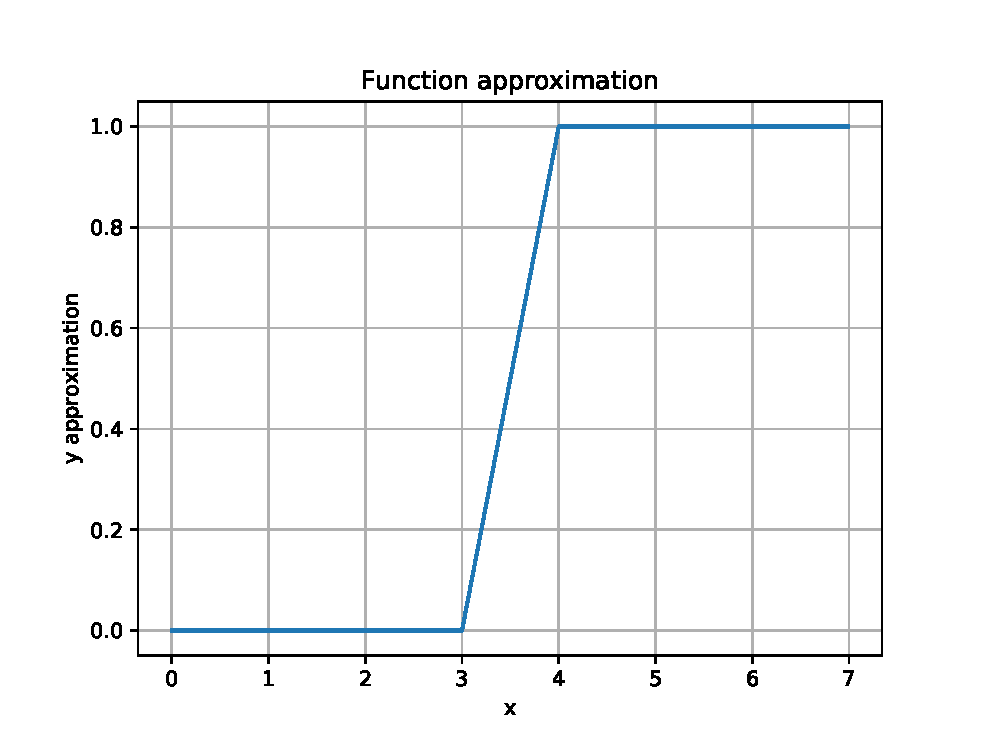
\includegraphics[scale=1]{graph.eps}
\caption{h(x)}
\end{figure}
We can notice that the function 
$h(x) = \max(0, x-3) - \max(0, x - 4)$.For $x<3$ function is 0, for $x> 4$ function is $x-4 + x-3 = 1$ and for $3\leq x\leq4$  is $x-3$In points $3$ and $4$ it has values $0$ and $1$.
\item[3.]
By setting $b_0^2=-c, b_1^2=-d, b_0^3=0, w_{00}^2=1, w_{10}^2=1, w_{00}^3=\frac{1}{d-c}, w_{01}^3=-\frac{1}{d-c}$ we get 
\begin{align*}
\hat{y} = \frac{\max(0, x-c)}{d-c} - \frac{\max(0, x-d)}{d-c}.
\end{align*} 
For $x<c, \hat{y}=0$. 
For $c\leq x\leq d$ $\hat{y}=\frac{x-c}{d-c}=\frac{1}{d-c}x - \frac{c}{d-c}$. For $x > d$ we have $\frac{x-c - (x - d)}{d-c}=1$
\item[4.]
First, let us prove that the $[0, 1]$ can be divided on a finite number of equal length subintervals where the difference between a minimum and maximum function value in that each interval is not bigger than $\varepsilon$.\\

According to the definition of the continuous function: given any $\varepsilon>0$, a $\delta>0$ can be found such that for every $x$ within the neighborhood of $x_0$ of radius $\delta$ ($|x-x_0|<\delta$) such that $|f(x)-f(x_0)|<\varepsilon$. 
Let us assume otherwise, that  $[0,1]$ cannot be divided into equal length intervals $[0, \delta, ..., \frac{1}{\delta}]$
whose $|f(x)-f(\frac{i\delta + (i+1)\delta}{2})|<\varepsilon$. 

This means no matter how small $\delta$ we set, there will always exist some $i$ such $|f(x)-f(\frac{i\delta + (i+1)\delta}{2})|\geq \varepsilon$, but this means as $\delta \rightarrow 0$ there will be always some value in $[0,1]$ interval that doesn't fulfill condition of continuality. Contradiction! \\
Thus, let us divide our $[0,1]$ interval into equal length subintervals with $\delta$ that such that   $$\left|f(x)-f\left(\frac{i\delta + (i+1)\delta}{2}\right)\right|<\varepsilon, i \in \left\{ 0, , \frac{1-\delta}{\delta}\right\}$$

We will prove that we can make a sliced linear function in such a way that it traverses through these limitations (which in reality are rectangles), and changes its shape at the beginning of each subinterval.
Because the function that we need to approximate is bounded and it can be negative, first, we will set $b_0^3$ such that $f(x)+b_0^3$ is always positive (in the worst case $b_0^3 = c$), this will be called $f_{positive}$. This means our sliced function has only to approximate positive bounded function. Moreover, if we concentrate on one specific rectangle (subinterval of function $f(x)$), we just need for a part of $h(x)$function to pass through it, so it starts in $f(i\delta)$ and it finishes in $f((i+1)\delta)$. 

\begin{lemma}
A unit in the hidden layer can produce function such that it has values $0$ before some value $x_0\geq0$ and it behaves as any linear function that passes through $x_0$ after  that. 
\end{lemma}

\begin{proof}
Let us denote with $w$ an input weight to this hidden unit, and $b$ a bias and $w_o$ weight to the output layer of this unit.
For a linear function $kx+n$ to pass through $x_0$: $kx_0 +n = 0$, $k= -\frac{n}{x_0}$.
Thus we can set $k$ to be positive as much as we want by setting $n$ to negative values.
This is easily achieved by setting $b=-kx_0$ and setting $w=k$ as we want, and setting $w_o=1$. This only works for $k\geq 0$. If we need to set $k\leq 0$, we  use the same trick with absolute value of $k$ and set $w_0$ to $-1$.
Thus  $b=-|k|x_0, w=|k|, w_o=sgn(k), k\neq0$, in the second case $ b=|c|, w=0, w_o=sgn(c), k=0$.
\end{proof}

Using lemma 1 we can just adjust the flow of our function so they "adjust" current linear function so it starts in $f(i\delta)$ and ends in $f((i+1)\delta)$.
For the first interval using lemma 1 $k = \frac{f(\delta) - f(0)}{\delta}$ and we should increase $b_0^3$ so that $h(0)=f_{positive}(0)$. So until the "end" of the first subinterval our function is in the $\varepsilon$ limits of $f(x)$. When it enters the second subinterval, we need to correct its coefficient in the following way:
if the desired coefficient for new subinterval is $k_r$ than $k$ in a new unit is $k_r - k_{previous}$, because 
$(k_r - k_{previous})x + k_{previous} = k_rx $. 
By applying this rule to every subinterval and generating new units in hidden layer consecutively, we will get the neural network that produces function $h(x)$, which approximates $f(x)$ in limit $\varepsilon$. 
\item[5.]
Let us notice:
\begin{align*}
\hat{y} = b_0^3 + \sum_{i=1}^N\max(0, b_i^2+w_{i0}^2x)w^3_{0i}
\end{align*}
If we notice that $ b_i^2+w_{i0}^2x$ are linear functions and they will only cut $x$ axis only once (unless they are parallel, but they won't cut the axis then, or in case when the line is axis, but then it won't have any influence on output because the value is 0). Thus, after the point of intersection (if one exists) their activation functions are either linear or constant. Because we have finite number of neurons, there is a maximal number $x$ in these cuts. After that point all functions will behave in the same way (either as linear function or constant). 
If we sum functions we will only have $a_ix + c_i$ and some constants. When we group coefficients next to $x$ and replace their sum with $m$ and the sum of constants and $b^3_0$ with $n$ we get the claim from the subproblem.
\item[6.]
I wouldn't invest for the following reasons. 
First, there is an infinite number of prime and composite numbers. Let us assume there is limited number of primes. If we multiple all primes and add 1 to the product, we will get number that is coprime to each of the primes, and thus each of the composite numbers. \\
The second, because the function, which is generated using types of NNs in this problem, after some time becomes linear (previous subproblem). They cannot derive anything from this function, because it is always increasing at the same pace, but number of prime numbers is unlimited, as the number of composite numbers.
\end{enumerate}
\end{enumerate}

\end{document}